% !TeX program = lualatex

\documentclass{beamer}

%! TeX root = dissertation.tex

\documentclass[11pt]{puthesis}

% packages
\usepackage{amsmath}
\usepackage{amssymb}
\usepackage[amsmath,thmmarks,noconfig]{ntheorem}
\usepackage{mathtools}
\usepackage{multirow}
\usepackage{pgfplots}
\usepackage{graphicx}
\usepackage{enumitem}
\usepackage{subcaption}
\usepackage{titlesec}
\usepackage{stackengine}
\usepackage{scalerel}
\usepackage{microtype}
\usepackage[boxruled,linesnumbered,commentsnumbered,procnumbered]{algorithm2e}
\usepackage[longnamesfirst]{natbib}
\usepackage[hypertexnames=false,hidelinks]{hyperref}
\usepackage[norefs,nocites]{refcheck}
\usepackage[defaultlines=4,all]{nowidow}
\usepackage{float}

% settings
\pgfplotsset{compat=1.9}
\newcommand{\TODO}[1]{\textcolor{red}{\textsc{TODO}: #1}}
\setcitestyle{round}
\captionsetup[subfigure]{justification=centering}

% tables numbered as figures
\def\table{\def\figurename{Table}\figure}
\let\endtable\endfigure
\renewcommand\listfigurename{Figures and Tables}

% arxiv references

% blackboard
\renewcommand{\P}{\ensuremath{\mathbb{P}}}
\newcommand{\N}{\ensuremath{\mathbb{N}}}
\newcommand{\R}{\ensuremath{\mathbb{R}}}
\newcommand{\E}{\ensuremath{\mathbb{E}}}
\newcommand{\Q}{\ensuremath{\mathbb{Q}}}
\newcommand{\I}{\ensuremath{\mathbb{I}}}
\newcommand{\Z}{\ensuremath{\mathbb{Z}}}

% roman
\newcommand{\rF}{\ensuremath{\mathrm{F}}}
\newcommand{\rH}{\ensuremath{\mathrm{H}}}
\newcommand{\rL}{\ensuremath{\mathrm{L}}}
\newcommand{\rk}{\ensuremath{\mathrm{k}}}
\newcommand{\rd}{\ensuremath{\mathrm{d}}}
\newcommand{\comp}{\ensuremath{\mathrm{c}}}
\newcommand{\TV}{\mathrm{TV}}

% bold
\newcommand{\bW}{\ensuremath{\mathbf{W}}}
\newcommand{\bY}{\ensuremath{\mathbf{Y}}}
\newcommand{\bX}{\ensuremath{\mathbf{X}}}
\newcommand{\bT}{\ensuremath{\mathbf{T}}}
\newcommand{\bA}{\ensuremath{\mathbf{A}}}
\newcommand{\bV}{\ensuremath{\mathbf{V}}}

% calligraphic
\newcommand{\cH}{\ensuremath{\mathcal{H}}}
\newcommand{\cF}{\ensuremath{\mathcal{F}}}
\newcommand{\cN}{\ensuremath{\mathcal{N}}}
\newcommand{\cX}{\ensuremath{\mathcal{X}}}
\newcommand{\cG}{\ensuremath{\mathcal{G}}}
\newcommand{\cW}{\ensuremath{\mathcal{W}}}
\newcommand{\cB}{\ensuremath{\mathcal{B}}}
\newcommand{\cS}{\ensuremath{\mathcal{S}}}
\newcommand{\cT}{\ensuremath{\mathcal{T}}}
\newcommand{\cV}{\ensuremath{\mathcal{V}}}
\newcommand{\cE}{\ensuremath{\mathcal{E}}}
\newcommand{\cU}{\ensuremath{\mathcal{U}}}
\newcommand{\cR}{\ensuremath{\mathcal{R}}}
\newcommand{\cA}{\ensuremath{\mathcal{A}}}
\newcommand{\cC}{\ensuremath{\mathcal{C}}}
\newcommand{\cM}{\ensuremath{\mathcal{M}}}
\newcommand{\cD}{\ensuremath{\mathcal{D}}}
\newcommand{\cP}{\ensuremath{\mathcal{P}}}
\newcommand{\cI}{\ensuremath{\mathcal{I}}}
\newcommand{\cY}{\ensuremath{\mathcal{Y}}}

% sans serif
\newcommand{\T}{\ensuremath{\mathsf{T}}}

% symbols
\newcommand{\vvvert}{{\vert\kern-0.25ex\vert\kern-0.25ex\vert}}
\newcommand{\bigvvvert}{{\big\vert\kern-0.35ex\big\vert\kern-0.35ex\big\vert}}
\newcommand{\Bigvvvert}{{\Big\vert\kern-0.3ex\Big\vert\kern-0.3ex\Big\vert}}
\newcommand{\bigsetminus}{\mathbin{\big\backslash}}
\newcommand{\Bigsetminus}{\mathbin{\Big\backslash}}
\newcommand{\dprime}{\ensuremath{\prime\prime}}
\newcommand{\tprime}{\ensuremath{\prime\prime\prime}}
\newcommand{\objective}{\ensuremath{\mathrm{obj}}}
\newcommand{\Dl}{\ensuremath{D_{\textup{lo}}}}
\newcommand{\Du}{\ensuremath{D_{\textup{up}}}}

% floor of beta
\newcommand{\flbeta}{{\ThisStyle{%
      \ensurestackMath{\stackengine{-0.5\LMpt}{\SavedStyle \beta}%
        {\SavedStyle {\rule{3.7\LMpt}{0.3\LMpt}}}
{U}{c}{F}{F}{S}}\vphantom{\beta}}}}

% operators
\DeclareMathOperator{\Var}{Var}
\DeclareMathOperator{\Cov}{Cov}
\DeclareMathOperator{\AIMSE}{AIMSE}
\DeclareMathOperator{\LOOCV}{LOOCV}
\DeclareMathOperator{\symconv}{symconv}
\DeclareMathOperator{\GCV}{GCV}
\DeclareMathOperator{\Unif}{Unif}
\DeclareMathOperator*{\logistic}{logistic}
\DeclareMathOperator{\Bias}{Bias}
\DeclareMathOperator{\Env}{Env}
\DeclareMathOperator*{\esssup}{ess\,sup}
\DeclareMathOperator{\Ber}{Ber}
\DeclareMathOperator{\KL}{KL}
\DeclareMathOperator{\Gam}{Gam}
\DeclareMathOperator{\Yule}{Yule}
\DeclareMathOperator{\rank}{rank}
\DeclareMathOperator{\Exp}{Exp}
\DeclareMathOperator{\Bin}{Bin}
\DeclareMathOperator{\Tr}{Tr}
\DeclareMathOperator{\Leb}{Leb}
\DeclareMathOperator*{\argmin}{arg\,min}
\DeclareMathOperator*{\minimize}{minimize}
\DeclareMathOperator*{\subjectto}{subject\ to}
\DeclareMathOperator{\IQR}{IQR}
\DeclareMathOperator{\ROT}{ROT}
\newcommand{\diff}[1]{\,\mathrm{d}#1}

% theorem environments
\renewtheoremstyle{break}{%
\item[\rlap{\vbox{\hbox{\hskip\labelsep \bfseries\upshape ##1\ %
  ##2}\hbox{\strut}}}]%
}{%
\item[\rlap{\vbox{\hbox{\hskip\labelsep \bfseries\upshape ##1\ %
  ##2\ \normalfont (##3)}\hbox{\strut}}}]%
}
\theoremstyle{break}
\theorempreskip{7mm}
\newtheorem{theorem}{Theorem}[section]
\newtheorem{lemma}{Lemma}[section]
\newtheorem{assumption}{Assumption}[section]
\newtheorem{corollary}{Corollary}[section]
\newtheorem{proposition}{Proposition}[section]
\newtheorem{definition}{Definition}[section]
\newtheorem{remark}{Remark}[section]

% proof environments
\let\proof\relax
\newtheoremstyle{proof}{%
\item[\rlap{\vbox{\hbox{\hskip\labelsep \bfseries\upshape ##1\ %
  }\hbox{\strut}}}]%
}{%
\item[\rlap{\vbox{\hbox{\hskip\labelsep \bfseries\upshape ##1\ %
  \normalfont (##3)}\hbox{\strut}}}]%
}
\theoremstyle{proof}
\theorembodyfont{\upshape}
\theorempreskip{7mm}
\theoremsymbol{\ensuremath{\square}}
\newtheorem{proof}{Proof}
\AtBeginEnvironment{proof}{\setcounter{proofparagraphcounter}{0}}%

% proof paragraphs
\titleformat{\paragraph}[hang]{\bfseries\upshape}{}{0pt}{}[]
\titlespacing*{\paragraph}{0pt}{6pt}{0pt}
\newcounter{proofparagraphcounter}
\newcommand{\proofparagraph}[1]{
  \refstepcounter{proofparagraphcounter}%
\paragraph{Part \theproofparagraphcounter : #1}}%

% inline roman lists
\newlist{inlineroman}{enumerate*}{1}
\setlist[inlineroman]{afterlabel=~,label=(\roman*)}

% algorithms
\DontPrintSemicolon%
\makeatletter%
\renewcommand{\SetKwInOut}[2]{%
  \sbox\algocf@inoutbox{\KwSty{#2}\algocf@typo:}%
  \expandafter\ifx\csname InOutSizeDefined\endcsname\relax%
  \newcommand\InOutSizeDefined{}%
  \setlength{\inoutsize}{\wd\algocf@inoutbox}%
  \sbox\algocf@inoutbox{%
    \parbox[t]{\inoutsize}%
    {\KwSty{#2}\algocf@typo:\hfill}~%
  }%
  \setlength{\inoutindent}{\wd\algocf@inoutbox}%
  \else%
  \ifdim\wd\algocf@inoutbox>\inoutsize%
  \setlength{\inoutsize}{\wd\algocf@inoutbox}%
  \sbox\algocf@inoutbox{%
    \parbox[t]{\inoutsize}%
    {\KwSty{#2}\algocf@typo:\hfill}~%
  }%
  \setlength{\inoutindent}{\wd\algocf@inoutbox}%
  \fi%
  \fi%
  \algocf@newcommand{#1}[1]{%
    \ifthenelse{\boolean{algocf@inoutnumbered}}{\relax}{\everypar={\relax}}{%
      \let\\\algocf@newinout\hangindent=\inoutindent\hangafter=1\parbox[t]%
      {\inoutsize}{\KwSty{#2}%
      \algocf@typo:\hfill}~##1\par%
    }%
    \algocf@linesnumbered%
  }%
}%
\makeatother%
\SetKwInOut{Input}{Input}%
\SetKwInOut{Output}{Output}%
\setlength{\algomargin}{2em}%


\definecolor{drycolor}{HTML}{ca5200}
\definecolor{wetcolor}{HTML}{0080d0}
\definecolor{currentcolor}{HTML}{8c19cf}
\definecolor{leafcolor}{HTML}{0aa00a}
\colorlet{alertcolor}{orange!65!black}

\title{
  Estimation and Inference in \\
  Modern Nonparametric Statistics%
  \vspace*{-2mm}
}

\author[shortname]{\textbf{William G.\ Underwood}}

\institute{
  Department of Operations Research and Financial Engineering \\
  Princeton University
}

\date{Final Public Oral Examination | May 7th, 2024}

\begin{document}
\NoHyper

\begin{frame}[noframenumbering,plain]{}
  \titlepage
\end{frame}

\begin{frame}{Research overview}

  \vspace*{2mm}

  Some of my recent work consists of

  \begin{itemize}
    \item \alert{Inference and estimation with Mondrian random forests}
      \nocite{cattaneo2023inference}
    \item \alert{Uniform inference for dyadic kernel density estimators}
      \nocite{cattaneo2024uniform}
    \item Yurinskii's coupling for martingales
      \nocite{cattaneo2022yurinskii}
  \end{itemize}

\end{frame}

\begin{frame}{Why random forests?}

  \vspace*{3mm}
  \begin{figure}[ht]
    \centering
    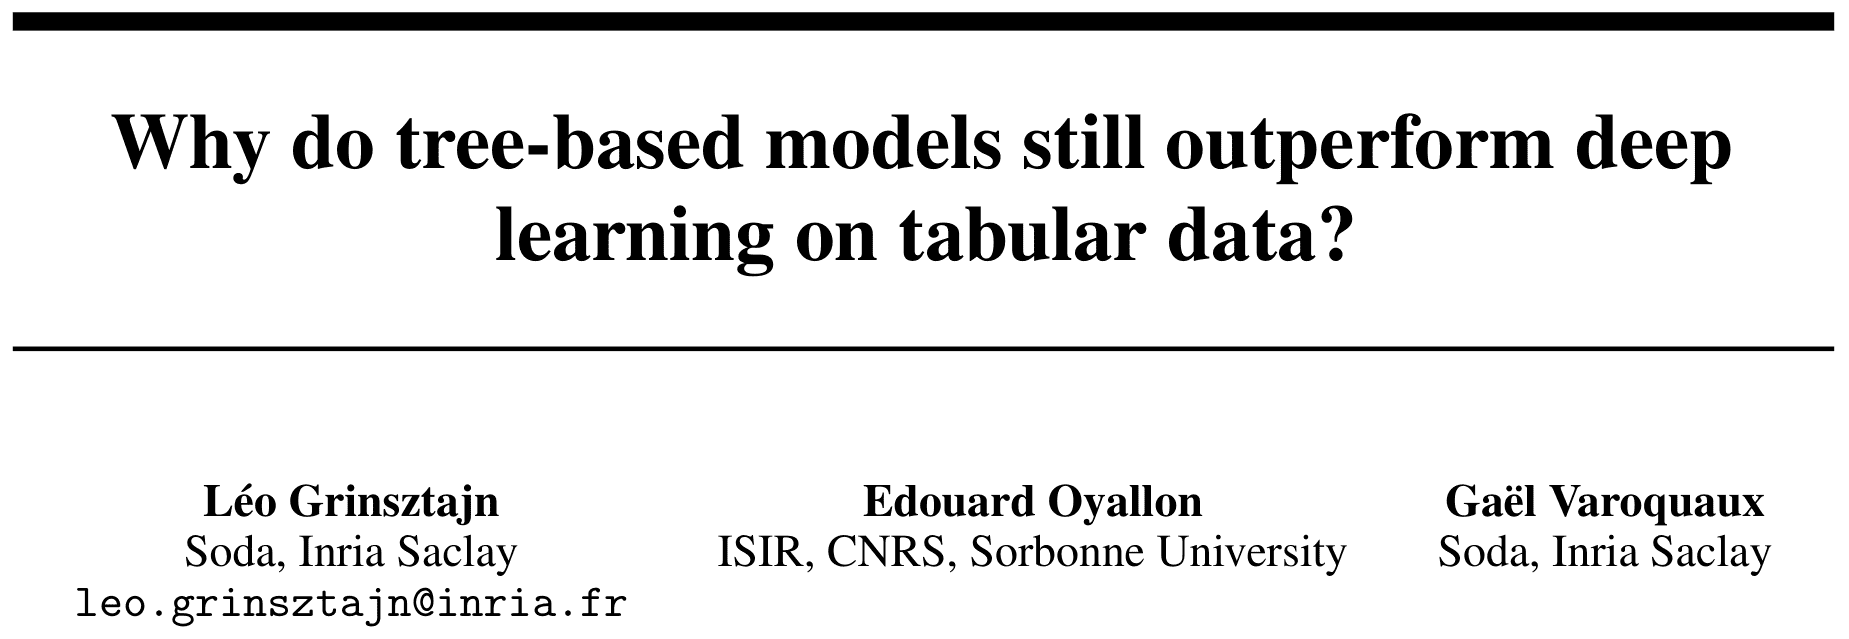
\includegraphics[scale=0.1]{graphics/forest_nn_paper.png}
  \end{figure}
  \vspace*{-1mm}

  \begin{itemize}

    \item Ensemble methods
      for regression and classification,
      with good performance, flexibility, robustness and efficiency
      \nocite{breiman2001random}
      \nocite{cutler2001pert}
      \nocite{breiman2004consistency}
      \nocite{geurts2006extremely}
      \nocite{menze2011oblique}
      \nocite{lakshminarayanan2014mondrian}

    \item
      Many variants including the popular ``Random Forest''

    \item
      Estimation theory has developed rapidly
      in recent years but
      applicability to statistical inference
      is less well understood

    \item
      In joint work with Matias D.\ Cattaneo and Jason M.\ Klusowski, \\
      I develop \alert{valid feasible inference} procedures
      and \alert{minimax optimal estimation} results
      for Mondrian random forests

  \end{itemize}

\end{frame}

\begin{frame}{Setup}

  Nonparametric regression setting

  \begin{itemize}
    \item Data $(X_i, Y_i)$ in $[0,1]^d \times \R$
      i.i.d.\ for $1 \leq i \leq n$
    \item $Y_i = \mu(X_i) + \varepsilon_i$
      with $\E[\varepsilon_i \mid X_i] = 0$
    \item Aim is to estimate and perform inference
      on unknown $\mu(x)$
  \end{itemize}

  Random forest regression estimators

  \begin{enumerate}
    \item Form a \alert{partition} of $[0,1]^d$,
      usually using a tree structure
    \item Fit constant estimates of $\mu$ on each cell in the partition
    \item Repeat with different partitions and \alert{average} the estimates
  \end{enumerate}
\end{frame}

\begin{frame}{Motivating example: weather forecasting in Australia}

  \begin{textblock*}{63mm}(60mm,20mm)
    \begin{itemize}
      \item<1> Weather data from Australian Bureau of Meteorology
        \nocite{bureau2017daily}
      \item<1> Rainfall from 2007--2017 at 49 locations
        with 125\,927 samples
      \item<1> Predict \textcolor{drycolor}{dry} or
        \textcolor{wetcolor}{wet} tomorrow
        with humidity and pressure today
      \item<1> Random forest classification
    \end{itemize}
  \end{textblock*}

  \begin{figure}
    \centering
    \hspace*{-13mm}
    \begin{subfigure}{0.54\textwidth}
      \centering
      \visible<1->{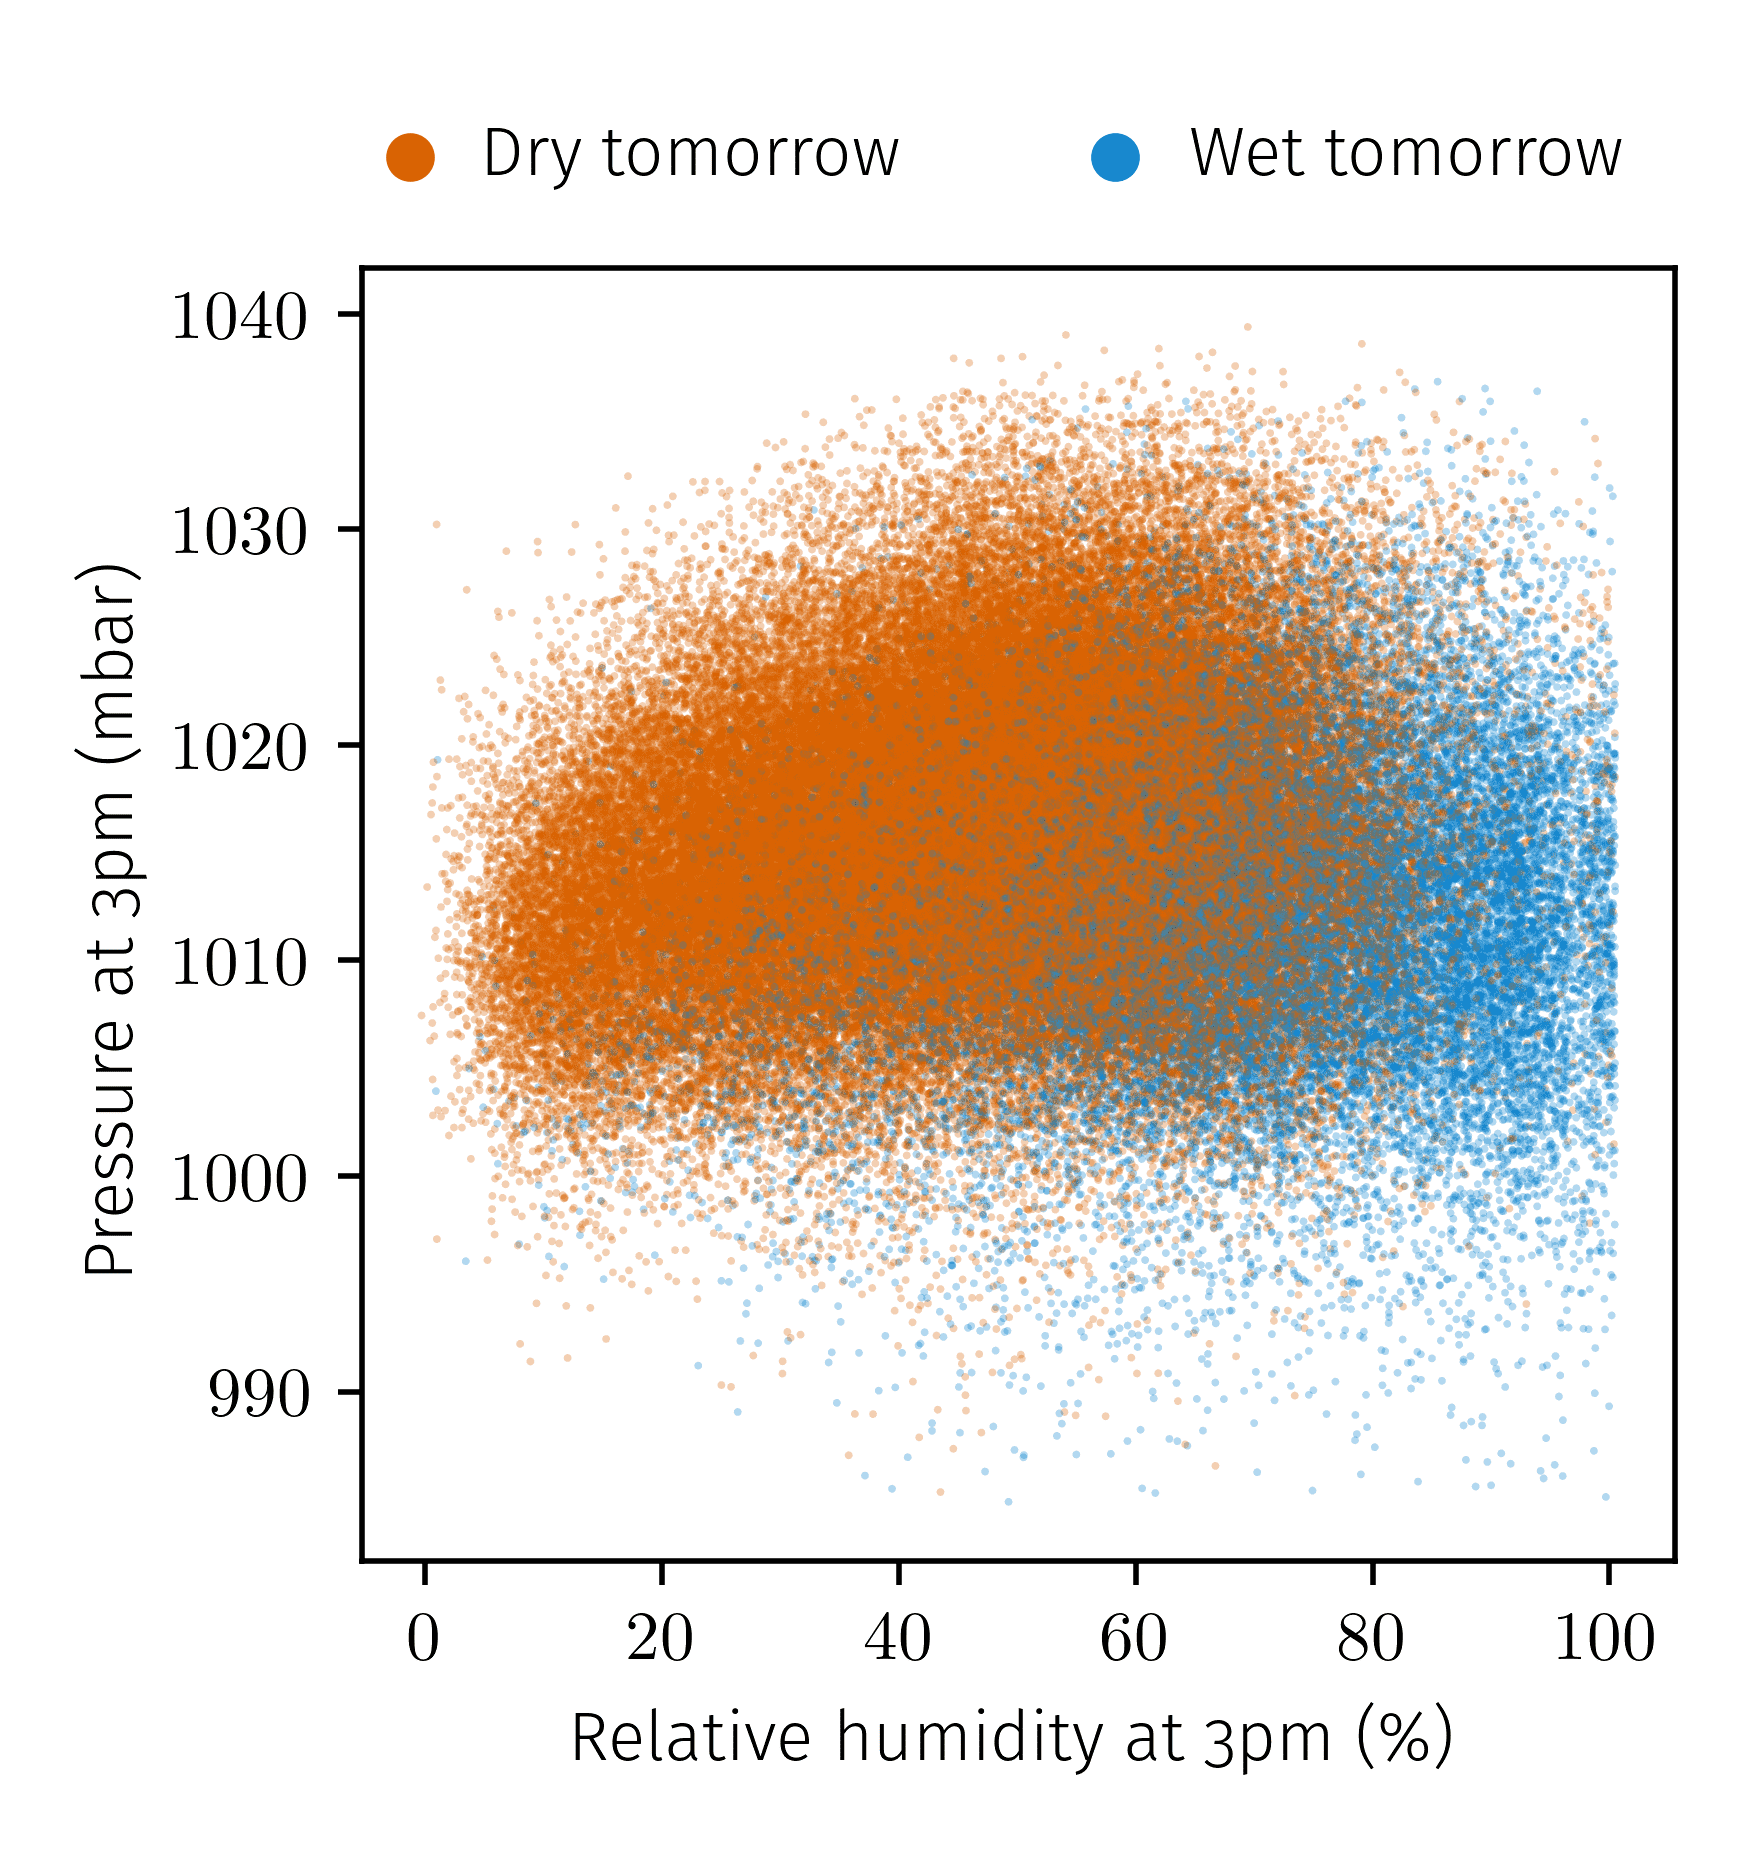
\includegraphics[scale=0.68]{
      graphics/weather_data.png}}%
    \end{subfigure}
    \begin{subfigure}{0.45\textwidth}
      \centering
      \visible<2->{%
        \includegraphics<1-2>[scale=0.68]{
        graphics/weather_data_partition.png}%
        \includegraphics<3>[scale=0.68]{
        graphics/weather_data_filled_partition.png}%
        \includegraphics<4>[scale=0.68]{
        graphics/weather_filled_partition_1.png}%
        \includegraphics<5>[scale=0.68]{
        graphics/weather_filled_partition_3.png}%
        \includegraphics<6>[scale=0.68]{
        graphics/weather_forest_2.png}%
        \includegraphics<7>[scale=0.68]{
        graphics/weather_forest_10.png}%
        \includegraphics<8>[scale=0.68]{
        graphics/weather_forest_30.png}%
      }
    \end{subfigure}
  \end{figure}

  \vspace*{-2mm}

  \begin{itemize}
      \visible<2->{%
        \only<1-2>{%
        \item First generate a partition of the predictor space
        }%
        \only<3>{%
        \item Compute average response in each cell with
          \textcolor{drycolor}{dry}$\ =0$, \textcolor{wetcolor}{wet}$\ =1$
        }%
        \only<4>{%
        \item This gives a single tree estimator of $\mu(x)$
        }%
        \only<5>{%
        \item Repeat with a different partition
        }%
        \only<6>{%
        \item Average predictions across 2 partitions
        }%
        \only<7>{%
        \item Average predictions across 10 partitions
        }%
        \only<8>{%
        \item Average across 30 partitions to get a random forest $\hat\mu(x)$
        }%
      }%
  \end{itemize}

\end{frame}

\begin{frame}{The Mondrian process}

  \vspace*{1mm}
  \begin{itemize}
    \item Rectangular partitions
      sampled from a Mondrian process \\
      \citep{roy2008mondrian}, write
      $T \sim \MP\big([0,1]^d, \lambda\big)$
    \item Tree complexity is controlled by the
      \alert{lifetime parameter} $\lambda > 0$
    \item The expected number of cells in $T$ is $(1+\lambda)^d$
    \item Mondrian random forests popular recently
      (Mourtada, Ga{\"\i}ffas and Scornet,
      NeurIPS 2017, AoS 2020, JRSSSB 2021)
  \end{itemize}

  \begin{figure}[ht]
    \centering
    \begin{subfigure}{0.4\textwidth}
      \centering
      
\includegraphics[scale=0.7]{graphics/piet_mondrian.png}%
      \caption*{A typical two-dimensional \\
      Mondrian partition with $\lambda = 4$}
    \end{subfigure}
    \hspace*{10mm}
    \begin{subfigure}{0.4\textwidth}
      \centering
      \setlength{\fboxsep}{0pt}%
      \setlength{\fboxrule}{0.28mm}%
      \fbox{
\includegraphics[scale=0.224]{graphics/piet.jpg}}%
      \caption*{Composition II in Red, Blue, \\ and Yellow, Piet Mondrian, 1930}
    \end{subfigure}
  \end{figure}

\end{frame}

\begin{frame}{Sampling a partition from the Mondrian process}

  \begin{textblock*}{100mm}(15mm,9mm)
    \begin{figure}[ht]
      \centering
      \hspace*{-16mm}
      \begin{subfigure}{0.5\textwidth}
        \centering
        \foreach \n in {1,...,12}{%
          \includegraphics<\n>[scale=0.9]{graphics/mondrian_process_\n.png}%
        }
      \end{subfigure}
      \hspace*{5mm}
      \begin{subfigure}{0.4\textwidth}
        \centering%
        \foreach \n in {1,...,12}{%
          \includegraphics<\n>[scale=0.9]{graphics/mondrian_tree_\n.png}%
        }
      \end{subfigure}
    \end{figure}
  \end{textblock*}

  \vspace*{54mm}
  \begin{itemize}
      \only<1>{%
      \item Fix $\lambda = 2$ and set $t=0$.
        The \alert{root cell} is $C_\emptyset = [0,1]^d$ with $d=2$
      \item We make recursive axis-aligned splits to generate a partition
      \item The lifetime parameter $\lambda$ determines when to stop splitting
      \item For any cell $C$, let $|C|_1 = \sum_{j=1}^{d} |C_j|$
        be the half-perimeter
      }%
      \only<2>{%
      \item Decide whether to split cell
        \textcolor{currentcolor}{$C_\emptyset$}
      \item Sample $E \sim \Exp(|C_\emptyset|_1)$, so $\E[E] = 1/|C_\emptyset|$
      \item Get $t + E \leq \lambda$ so
        \textcolor{currentcolor}{$C_\emptyset$} is split
      }%
      \only<3>{%
      \item Choose split axis by
        $\P(J = j) = \frac{|C_{\emptyset j}|}{|C_\emptyset|_1}$, get $J = 1$
      \item Select split location by $S \sim \Unif(C_{\emptyset J})$
      \item Replace \textcolor{currentcolor}{$C_\emptyset$} by
        $C_\LL = \{x \in C: x_J \leq S\}$
        and $C_\RR = C \setminus C_\LL$
      }%
      \only<4>{%
      \item Decide whether to split cell
        \textcolor{currentcolor}{$C_{\mathrm L}$}
      \item Sample $E \sim \Exp(|C_{\mathrm L}|_1)$
      \item Get $t + E \leq \lambda$ so
        \textcolor{currentcolor}{$C_{\mathrm L}$} is split
      }%
      \only<5>{%
      \item Choose split axis by
        $\P(J = j) = \frac{|C_{\mathrm L j}|}{|C_\mathrm L|_1}$, get $J = 2$
      \item Select split location by $S \sim \Unif(C_{\mathrm L J})$
      \item Replace \textcolor{currentcolor}{$C_{\mathrm L}$} by
        $C_{\mathrm{LL}} = \{x \in C_{\mathrm L}: x_J \leq S\}$
        and $C_\mathrm{LR} = C_\mathrm{L} \setminus C_\mathrm{LL}$
      }%
      \only<6>{%
      \item Decide whether to split cell
        \textcolor{currentcolor}{$C_{\mathrm R}$}
      \item Sample $E \sim \Exp(|C_{\mathrm R}|_1)$
      \item Get $t + E > \lambda$ so \textcolor{currentcolor}{$C_{\mathrm R}$}
        is not split and becomes a \textcolor{leafcolor}{leaf}
      }%
      \only<7>{%
      \item We continue this process
      }%
      \only<8>{%
      \item \textcolor{currentcolor}{$C_\mathrm{LL}$} is split
        on axis $2$
      }%
      \only<9>{%
      \item
        \textcolor{currentcolor}{$C_{\mathrm{LR}}$} is not split
        and becomes a \textcolor{leafcolor}{leaf}
      }%
      \only<10>{%
      \item
        \textcolor{currentcolor}{$C_{\mathrm{LLL}}$}
        becomes a \textcolor{leafcolor}{leaf}
      }%
      \only<11>{%
      \item
        \textcolor{currentcolor}{$C_{\mathrm{LLR}}$}
        becomes a \textcolor{leafcolor}{leaf}
      }%
      \only<12>{%
      \item All cells are now \textcolor{leafcolor}{leaves}, and the sampling is
        complete
      \item To increase $\lambda$ we continue this process, allowing
        \alert{online fitting}
      \item Australian weather data:
        rescaled to $[0,1]^2$ and set $\lambda = 5$
      }%
  \end{itemize}

\end{frame}

\begin{frame}{Properties of the Mondrian process}

  \begin{minipage}{0.62\textwidth}
    \vspace*{-2mm}
    \begin{beamerlemma}[Cell shape distribution]
      Let $T \sim \MP\big([0,1]^d, \lambda\big)$,
      take $x \in [0,1]^d$
      and write $T(x)$ for the cell containing $x$.
      With $E_{j1}$ and $E_{j2}$ independent
      $\Exp(\lambda)$,
      %
      \vspace*{-3mm}
      \begin{align*}
        T(x) =
        [0,1]^d \cap
        \prod_{j=1}^{d}
        \big[
          x_j - E_{j1},
          x_j + E_{j2}
        \big]
      \end{align*}
      \vspace*{-4mm}
    \end{beamerlemma}
  \end{minipage}
  \begin{minipage}{0.0\textwidth}
    \phantom{spacing}
  \end{minipage}
  \begin{minipage}{0.3\textwidth}
    \vspace*{3mm}
    \begin{figure}[ht]
      \centering
      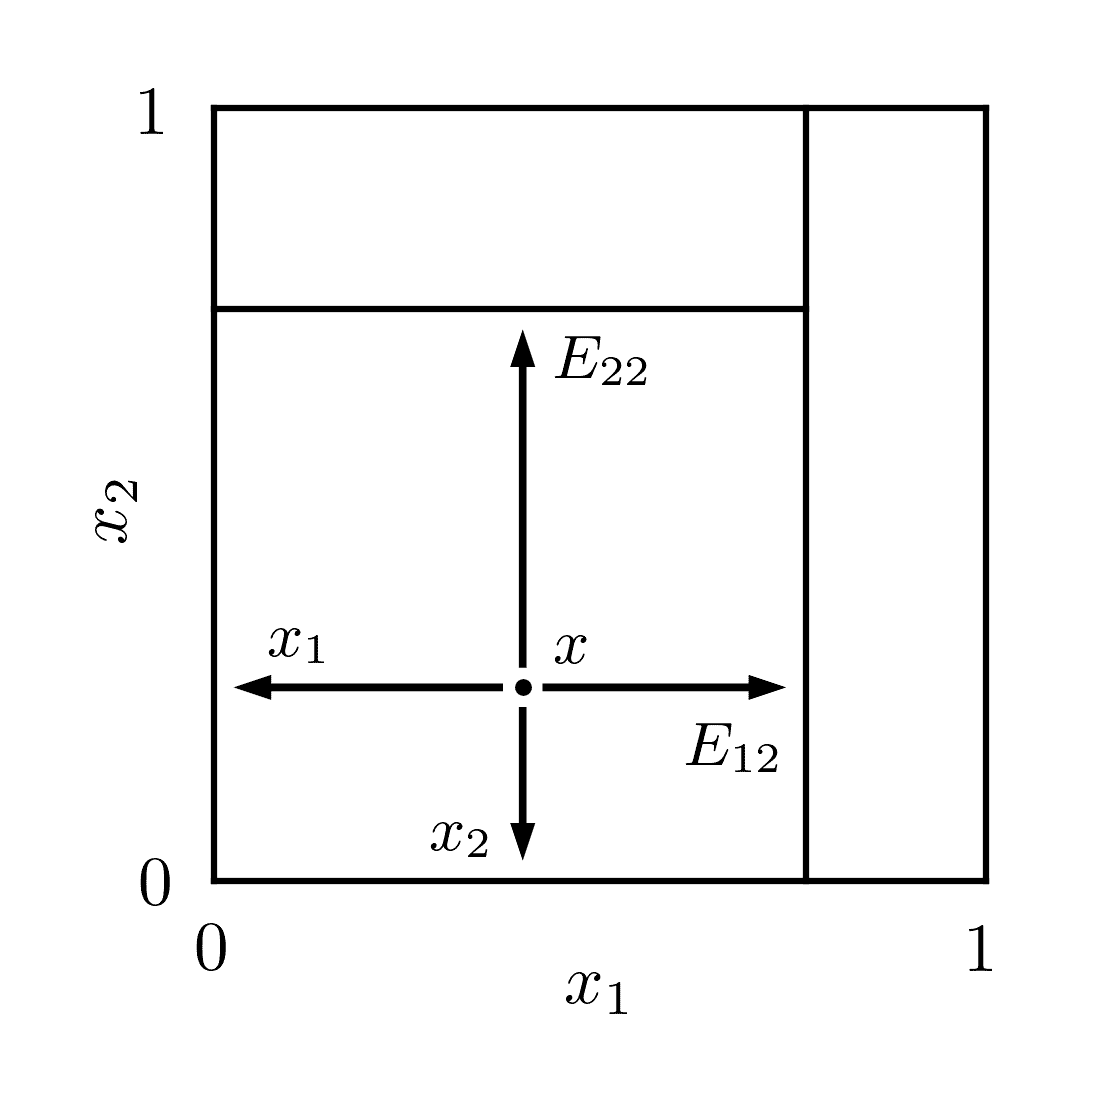
\includegraphics[scale=0.85]{graphics/theorem_distribution.png}
    \end{figure}
  \end{minipage}

  \begin{itemize}
    \item
      Roy and Teh (NeurIPS 2008);
      Mourtada, Ga{\"\i}ffas and Scornet
      (NeurIPS 2017, AoS 2020, JRSSSB 2021)
      \nocite{roy2008mondrian}
      \nocite{mourtada2017universal}
      \nocite{mourtada2020minimax}
      \nocite{mourtada2021amf}
    \item With $d=1$, have a Poisson process
      on $[0,1]$ with intensity $\lambda$
    \item The smallest cell is much smaller than
      the average cell
  \end{itemize}
\end{frame}

\begin{frame}{Mondrian random forests}

  \vspace*{4mm}
  \begin{itemize}
    \item Let $B$ be the desired number of trees in the forest
    \item Sample
      $T_1, \ldots, T_B \sim \MP\big([0,1]^d, \lambda\big)$
      \alert{independently}
    \item For each cell in $T_b$,
      compute the average $Y_i$ value
    \item Finally average across all the trees

    \item
      Writing $N_b(x) = \sum_{i=1}^n \I\big\{ X_i \in T_b(x) \big\}$
      for the number of data points in the same cell as $x$,
      and with $0/0 = 0$, we have
      %
      \vspace*{3mm}
      \begin{definition}[Mondrian random forest estimator]%
        \vspace*{-3mm}
        \begin{align*}
          \hat\mu(x)
          =
          \underbrace{
            \frac{1}{B} \sum_{b=1}^B
          }_{\text{\alert{Forest}}}
          \hspace*{1mm}
          \underbrace{
            \frac{1}{N_b(x)}
            \sum_{i=1}^n Y_i \,
            \I\big\{ X_i \in T_b(x) \big\}
            \vphantom{\frac{1}{B} \sum_{b=1}^B}
          }_{\text{\alert{Mean of $Y_i$ in cell containing $x$}}}
        \end{align*}
        \vspace*{-4mm}
      \end{definition}

  \end{itemize}

\end{frame}

\begin{frame}{Bias--variance decomposition}

  With $\bX = (X_1, \ldots, X_n)$ and
  $\bT = (T_1, \ldots, T_B)$,
  %
  \begin{align*}
    \hat \mu(x)
    - \mu(x)
    &=
    \underbrace{
      \hat \mu(x)
      - \E \big[ \hat \mu(x) \mid \bX, \bT \big]
    }_{\text{\textcolor{alertcolor}{Variance}}}
    + \underbrace{
      \E \big[ \hat \mu(x) \mid \bX, \bT \big]
      - \mu(x)
    }_{\text{\textcolor{currentcolor}{Bias}}}
  \end{align*}
  %
  \begin{enumerate}
    \item Derive a central limit theorem for the
      \textcolor{alertcolor}{variance}
      term
    \item Approximate the
      \textcolor{currentcolor}{bias}
      term in probability
    \item Perform inference by ensuring the bias is negligible
    \item Minimax optimal estimation with debiasing
  \end{enumerate}

\end{frame}

\begin{frame}{Assumptions on data and estimator}

  \vspace*{2mm}
  \begin{itemize}
    \item Recall $(X_i, Y_i)$ in $[0,1]^d \times \R$
      i.i.d.\ with $Y_i = \mu(X_i) + \varepsilon_i$
    \item $X_i$ has Lebesgue density
      $f$, bounded away from zero
    \item A version of
      $\sigma^2(X_i) = \E \left[ \varepsilon_i^2 \mid X_i \right]$
      is Lipschitz
    \item
      $\E \left[ \varepsilon_i^4 \mid X_i \right]$
      is bounded almost surely
    \item Both $\mu$ and $f$ are
      \alert{$\beta$-H{\"o}lder continuous}
      for some $\beta \geq 1$
    \item $x \in (0,1)^d$
      is an interior evaluation point
    \item
      $\frac{\lambda^d \log n}{n} \to 0$
      and
      $\log \lambda \asymp \log B \asymp \log n$,
      so $\lambda \to \infty$ and $B \to \infty$
  \end{itemize}

  %\vspace*{3mm}
  \begin{definition}[$\beta$-H{\"o}lder continuity]
    With $\flbeta$ the largest integer
    less than $\beta$, for all $x,x' \in [0,1]^d$,
    %
    \vspace*{-2mm}
    \begin{align*}
      \max_{|\nu| = \flbeta}
      \left|
      \partial^\nu \hspace*{-0.5mm} g(x)
      - \partial^{\nu} \hspace*{-0.5mm} g(x')
      \right|
      &\lesssim \|x-x'\|_2^{\beta - \flbeta}
    \end{align*}
    \vspace*{-4mm}
    %
  \end{definition}

\end{frame}

\begin{frame}{Central limit theorem for Mondrian random forests}

  \vspace*{3mm}
  \begin{beamertheorem}[Central limit theorem for Mondrian random forests]%
    \vspace*{-3mm}
    \begin{align*}
      \sqrt{\frac{n}{\lambda^d}}
      \Big(
        \hat \mu(x)
        - \E \big[ \hat \mu(x) \mid \bX, \bT \big]
      \Big)
      &\rightsquigarrow
      \cN\big(0, \Sigma(x)\big)
    \end{align*}
    \vspace*{-4mm}
    %
    where
    %
    \vspace*{-4mm}
    \begin{align*}
      \Sigma(x)
      &=
      \frac{\sigma^2(x)}{f(x)}
      \left(
        \frac{4 - 4 \log 2}{3 }
      \right)^d
    \end{align*}
    \vspace*{-4mm}
  \end{beamertheorem}

  \vspace*{-7mm}
  \begin{align*}
    \hat \mu(x)
    - \E \big[ \hat \mu(x) \mid \bX, \bT \big]
    &=
    \frac{1}{B} \sum_{b=1}^B
    \frac{1}{N_b(x)}
    \sum_{i=1}^n \varepsilon_i \,
    \I\big\{ X_i \in T_b(x) \big\}
  \end{align*}

  \vspace*{-1mm}
  \begin{itemize}
    \item
      Essential that $B \to \infty$, or randomness persists in the limit
    \item
      No conditional independence as $N_b(x)$ depends on all $X_i$
    \item
      Replacing $N_b(x)$ by $n f(x) |T_b(x)|$ fails
      as $\E \left[ \frac{1}{|T_b(x)|^2} \right] = \infty$
    \item
      Central limit theorems based on $2+\delta$ moments inadequate

  \end{itemize}

\end{frame}

\begin{frame}{Central limit theorem for Mondrian random forests}

  \begin{align*}
    \hat \mu(x)
    - \E \big[ \hat \mu(x) \mid \bX, \bT \big]
    &=
    \frac{1}{B} \sum_{b=1}^B
    \frac{1}{N_b(x)}
    \sum_{i=1}^n \varepsilon_i \,
    \I\big\{ X_i \in T_b(x) \big\}
  \end{align*}
  \vspace*{-3mm}
  %
  \begin{itemize}
      %
    \item Use a \alert{martingale central limit theorem}
      \citep{hall1980martingale}
    \item Take the filtration
      $\cF_{n i} =
      \sigma \left( \bX, \bT, \varepsilon_1, \ldots, \varepsilon_i \right)$
      and consider $\sum_{i=1}^n M_{n i}(x)$
      with the martingale differences
      %
      \begin{align*}
        M_{n i}(x)
        &=
        \sqrt{\frac{n}{\lambda^d}}
        \frac{1}{B} \sum_{b=1}^B
        \frac{1} {N_{b}(x)}
        \varepsilon_i \,
        \I\{X_i \in T_b(x)\}
      \end{align*}
      %
    \item
      Verify
      $\E\left[\max_{1 \leq i \leq n} M_{n i}(x)^2\right] \lesssim 1$
      and $\sum_{i=1}^n M_{n i}(x)^2 \to_\P \Sigma(x)$
    \item
      Nonlinear structure handled by
      the Efron--Stein inequality
  \end{itemize}

\end{frame}

\begin{frame}{Bias of Mondrian random forests}

  \vspace*{3mm}
  \begin{beamertheorem}[Bias of Mondrian random forests]%
    %
    There exist $B_r(x)$ depending only on $f$ and $\mu$ such that
    %
    \vspace*{-2mm}
    \begin{align*}
      \left|
      \E \big[ \hat \mu(x) \mid \bX, \bT \big]
      - \mu(x)
      - \hspace*{-1.5mm} \sum_{r=1}^{\lfloor \flbeta / 2 \rfloor}
      \hspace*{-0.5mm}
      \frac{B_r(x)}{\lambda^{2r}}
      \right|
      \lesssim_\P
      \frac{1}{\lambda^\beta}
      + \textcolor{alertcolor}{\frac{1}{\lambda \sqrt B}}
      + \frac{\log n}{\lambda} \sqrt{\frac{\lambda^d}{n}}
    \end{align*}
    \vspace*{-4mm}
    %
  \end{beamertheorem}

  \begin{itemize}

    \item We approximate the bias with a Taylor polynomial
      in $1/\lambda^2$
    \item If $B$ does not diverge
      there is a
      \alert{first-order bias}
      of size $1 / \lambda$

    \item In large forests and with $\beta \geq 2$,
      leading bias is of size $1 / \lambda^2$

    \item Setting
      $\lambda \asymp n^{\frac{1}{d + 4}}$
      and $B \gg n^{\frac{2}{d + 4}}$ gives
      for $\beta \geq 2$
      %
      \vspace*{3mm}
      \begin{align*}
        \Big| \hat \mu(x) - \mu(x) \Big|
        \lesssim_\P
        \underbrace{%
          \sqrt{\frac{\lambda^d}{n}}%
          \vphantom{\frac{1}{\lambda \sqrt B}}%
        }_{\alert{\text{Variance}}}
        \hspace*{-1mm}
        + \underbrace{
          \frac{1}{\lambda^2}
          + \frac{1}{\lambda \sqrt B}
        }_{\alert{\text{Bias}}}
        \lesssim
        n^{-\frac{2}{d+4}}
      \end{align*}

  \end{itemize}

\end{frame}

\begin{frame}{Inference with Mondrian random forests}

  \begin{itemize}
    \item
      Combine central limit theorem and bias bound for inference
    \item Bias is negligible if $\beta \geq 2$ and
      $\frac{1}{\lambda^2} + \frac{1}{\lambda \sqrt B}
      \ll \sqrt{\frac{\lambda^d}{n}}$
    \item We construct a variance estimator
      $\hat\Sigma(x) \to_\P \Sigma(x)$
    \item Let $q_{\alpha}$ be the
      $1 - \frac{\alpha}{2}$ quantile of $\cN(0,1)$
  \end{itemize}

  \vspace*{3mm}
  \begin{beamertheorem}[Feasible confidence intervals]%
    With $\beta \geq 2$,
    if $\lambda \gg n^{\frac{1}{d + 4}}$
    and $B \gg n^{\frac{2}{d + 4}}$ then
    \vspace*{-1mm}
    \begin{align*}
      \P \left(
        \mu(x) \in
        \left[
          \hat \mu(x)
          \pm \sqrt{\frac{\lambda^d}{n}} \hat \Sigma(x)^{1/2}
          q_{\alpha}
        \right]
      \right)
      \to
      1 - \alpha
    \end{align*}
    \vspace*{-3mm}
  \end{beamertheorem}

\end{frame}

\begin{frame}{Debiased Mondrian random forests}

  \vspace*{3mm}
  \begin{itemize}
    \item Bias approximation with $\beta > 2$
      for lifetimes $\lambda$ and $\textcolor{alertcolor}{2} \lambda$ gives
      %
      \begin{align}
        \E \big[ \hat \mu(x; \lambda) \mid \bX, \bT \big]
        &\approx
        \mu(x) + \tfrac{B_1(x)}{\lambda^2} \\
        \E \big[ \hat \mu(x; \textcolor{alertcolor}{2} \lambda)
        \mid \bX, \bT \big]
        &\approx
        \mu(x) + \tfrac{B_1(x)}{\textcolor{alertcolor}{4} \lambda^2}
      \end{align}

    \item Take a linear combination to annihilate the leading bias
      %
      \begin{align*}
        \E \left[
          \textcolor{currentcolor}{-\tfrac{1}{3}}
          \hat \mu(x; \lambda)
          +\textcolor{currentcolor}{\tfrac{4}{3}}
          \hat \mu(x; \textcolor{alertcolor}{2} \lambda)
        \mid \bX, \bT \right]
        &\approx
        \mu(x) + 0
      \end{align*}

    \item
      Cancel all
      $J = \lfloor \flbeta / 2 \rfloor$ bias terms
      to get the debiased estimator
      %
      \begin{align*}
        \hat \mu_\rd(x)
        &=
        \sum_{s=0}^J
        \textcolor{currentcolor}{\omega_s}
        \hat \mu(x;
          \textcolor{alertcolor}{a_s}
        \lambda)
      \end{align*}

    \item
      Here $\textcolor{alertcolor}{a_s}$ are fixed,
      and $\textcolor{currentcolor}{\omega_s}$ solve the linear equations \\
      $\sum_{s=0}^{J} \textcolor{currentcolor}{\omega_s} = 1$
      and $\sum_{s=0}^{J}
      \textcolor{currentcolor}{\omega_s}
      \textcolor{alertcolor}{a_s}^{-2r} = 0$
      for $1 \leq r \leq J$

  \end{itemize}

\end{frame}

\begin{frame}{Results for debiased Mondrian random forests}

  \vspace*{2mm}
  \begin{beamertheorem}[Improved bias bound]%
    \vspace*{-4mm}
    \begin{align*}
      \left|
      \E \big[ \hat \mu_\rd(x) \mid \bX, \bT \big]
      - \mu(x)
      \right|
      &\lesssim_\P
      \textcolor{alertcolor}{\frac{1}{\lambda^{\beta}}}
      + \frac{1}{\lambda \sqrt B}
      + \frac{\log n}{\lambda} \sqrt{\frac{\lambda^d}{n}}
    \end{align*}
    \vspace*{-5mm}
  \end{beamertheorem}

  \begin{beamertheorem}[Central limit theorem with debiasing]%
    \vspace*{-4mm}
    \begin{align*}
      \sqrt{\frac{n}{\lambda^d}}
      \Big(
        \hat \mu_\rd(x)
        - \E \big[ \hat \mu_\rd(x) \mid \bX, \bT \big]
      \Big)
      &\rightsquigarrow
      \cN\big(0, \textcolor{alertcolor}{\Sigma_\rd(x)}\big)
    \end{align*}
    \vspace*{-5mm}
  \end{beamertheorem}

  \begin{beamertheorem}[Feasible confidence intervals with debiasing]%
    If $\lambda \gg n^{\frac{1}{d + 2 \beta}}$
    and $B \gg n^{\frac{2 \beta - 2}{d + 2 \beta}}$,
    with $\hat\Sigma_\rd(x)$
    a variance estimator,
    \vspace*{-1mm}
    \begin{align*}
      \P \left(
        \mu(x) \in
        \left[
          \hat \mu_\rd(x)
          \pm \sqrt{\frac{\lambda^d}{n}} \hat \Sigma_\rd(x)^{1/2}
          q_{\alpha}
        \right]
      \right)
      \to
      1 - \alpha
    \end{align*}
    \vspace*{-3mm}
  \end{beamertheorem}

\end{frame}

\begin{frame}{Minimax optimality}

  \vspace*{3mm}
  \begin{beamertheorem}[Minimaxity of debiased
    Mondrian random forests]%
    If $\lambda \asymp n^{\frac{1}{d + 2 \beta}}$
    and $B \gtrsim n^{\frac{2 \beta - 2}{d + 2 \beta}}$,
    then
    %
    \begin{align*}
      \E \left[
        \big(
          \hat \mu_\rd(x)
          - \mu(x)
        \big)^2
      \right]^{1/2}
      &\lesssim
      \underbrace{\sqrt{\frac{\lambda^d}{n}}
        \vphantom{\frac{1}{\lambda \sqrt B}}
      }_{\text{\textcolor{alertcolor}{Variance}}}
      + \underbrace{\frac{1}{\lambda^\beta}
        + \frac{1}{\lambda \sqrt B}
      }_{\text{\textcolor{currentcolor}{Bias}}}
      \lesssim
      n^{-\frac{\beta}{d + 2 \beta}}
    \end{align*}
    %
    \vspace*{-3mm}
  \end{beamertheorem}

  \begin{table}
    \begin{center}
      \begin{tabular}{|c|c|}
        \hline
        \textbf{Estimator} & \textbf{Minimax condition} \\
        \hline
        Mondrian tree$^*$ &
        $\beta \in (0, 1]$ \\
        Mondrian random forest$^*$ &
        $\beta \in (0, 2]$ \\
        \alert{Debiased Mondrian random forest} &
        \hspace*{2mm}$\beta \in (0, \infty)$ \\
        \hline
      \end{tabular}
    \end{center}
  \end{table}
  \vspace*{1mm}

  $^*$Established by \citet{mourtada2020minimax}

\end{frame}

\begin{frame}{Example: weather forecasting in Australia}

  \vspace*{-2mm}
  \begin{figure}
    \centering
    \hspace*{-13mm}
    \begin{subfigure}{0.54\textwidth}
      \centering
      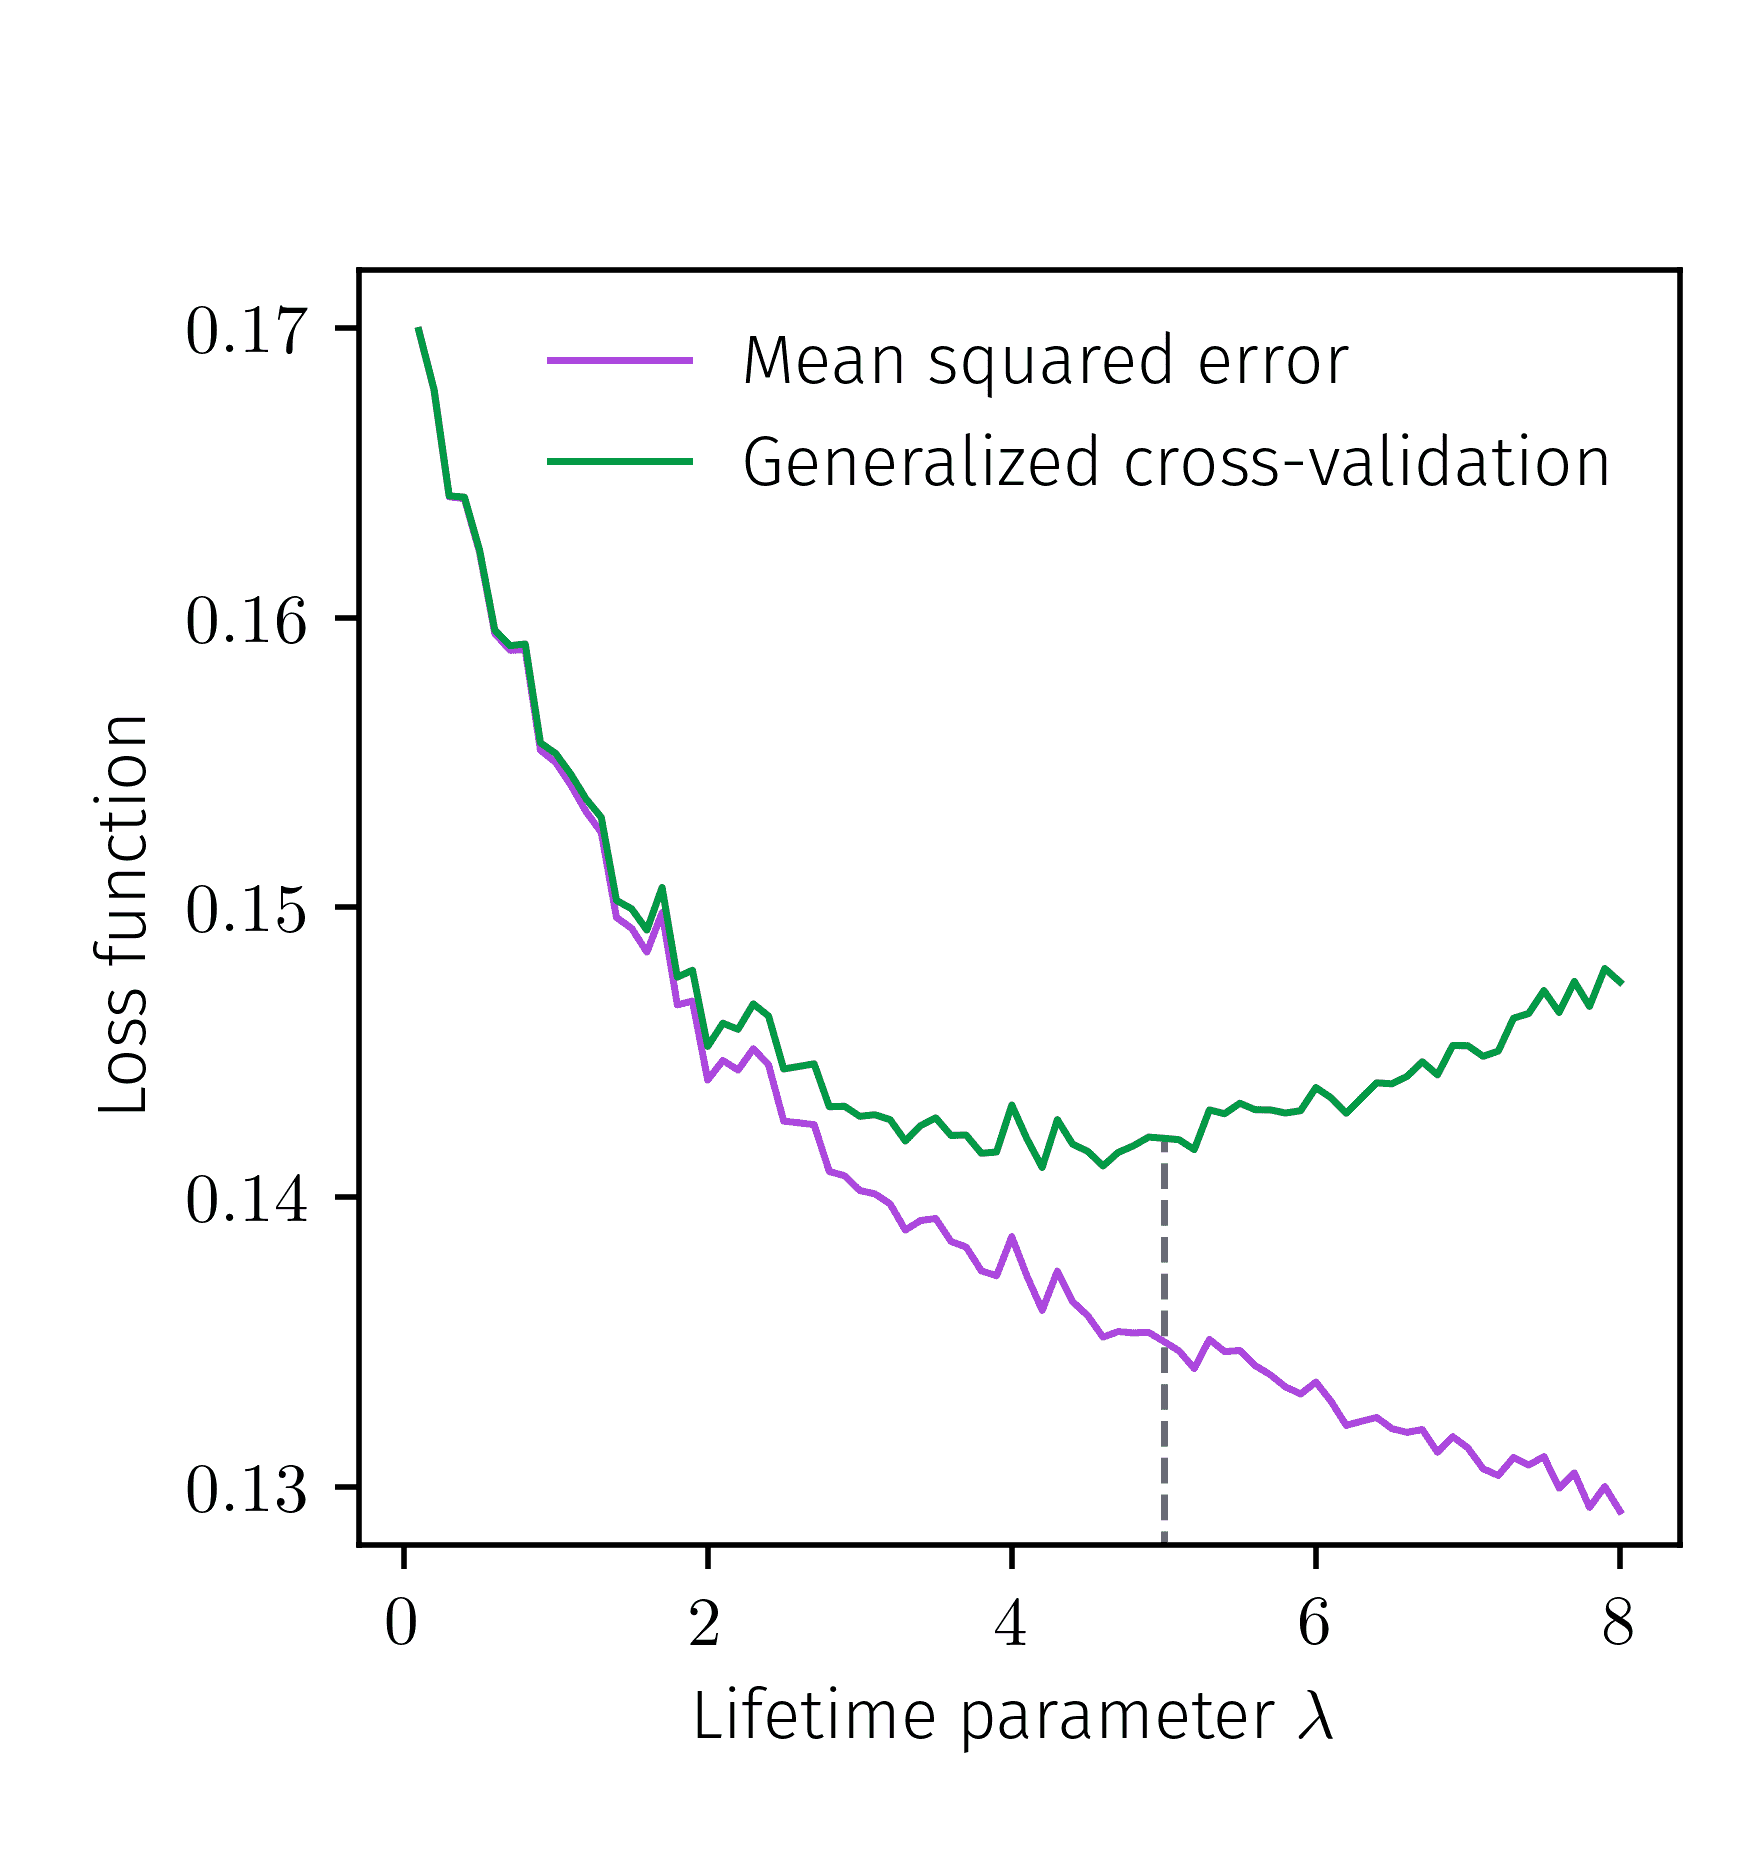
\includegraphics[scale=0.6]{
      graphics/weather_gcv.png}%
    \end{subfigure}
    \begin{subfigure}{0.45\textwidth}
      \centering
      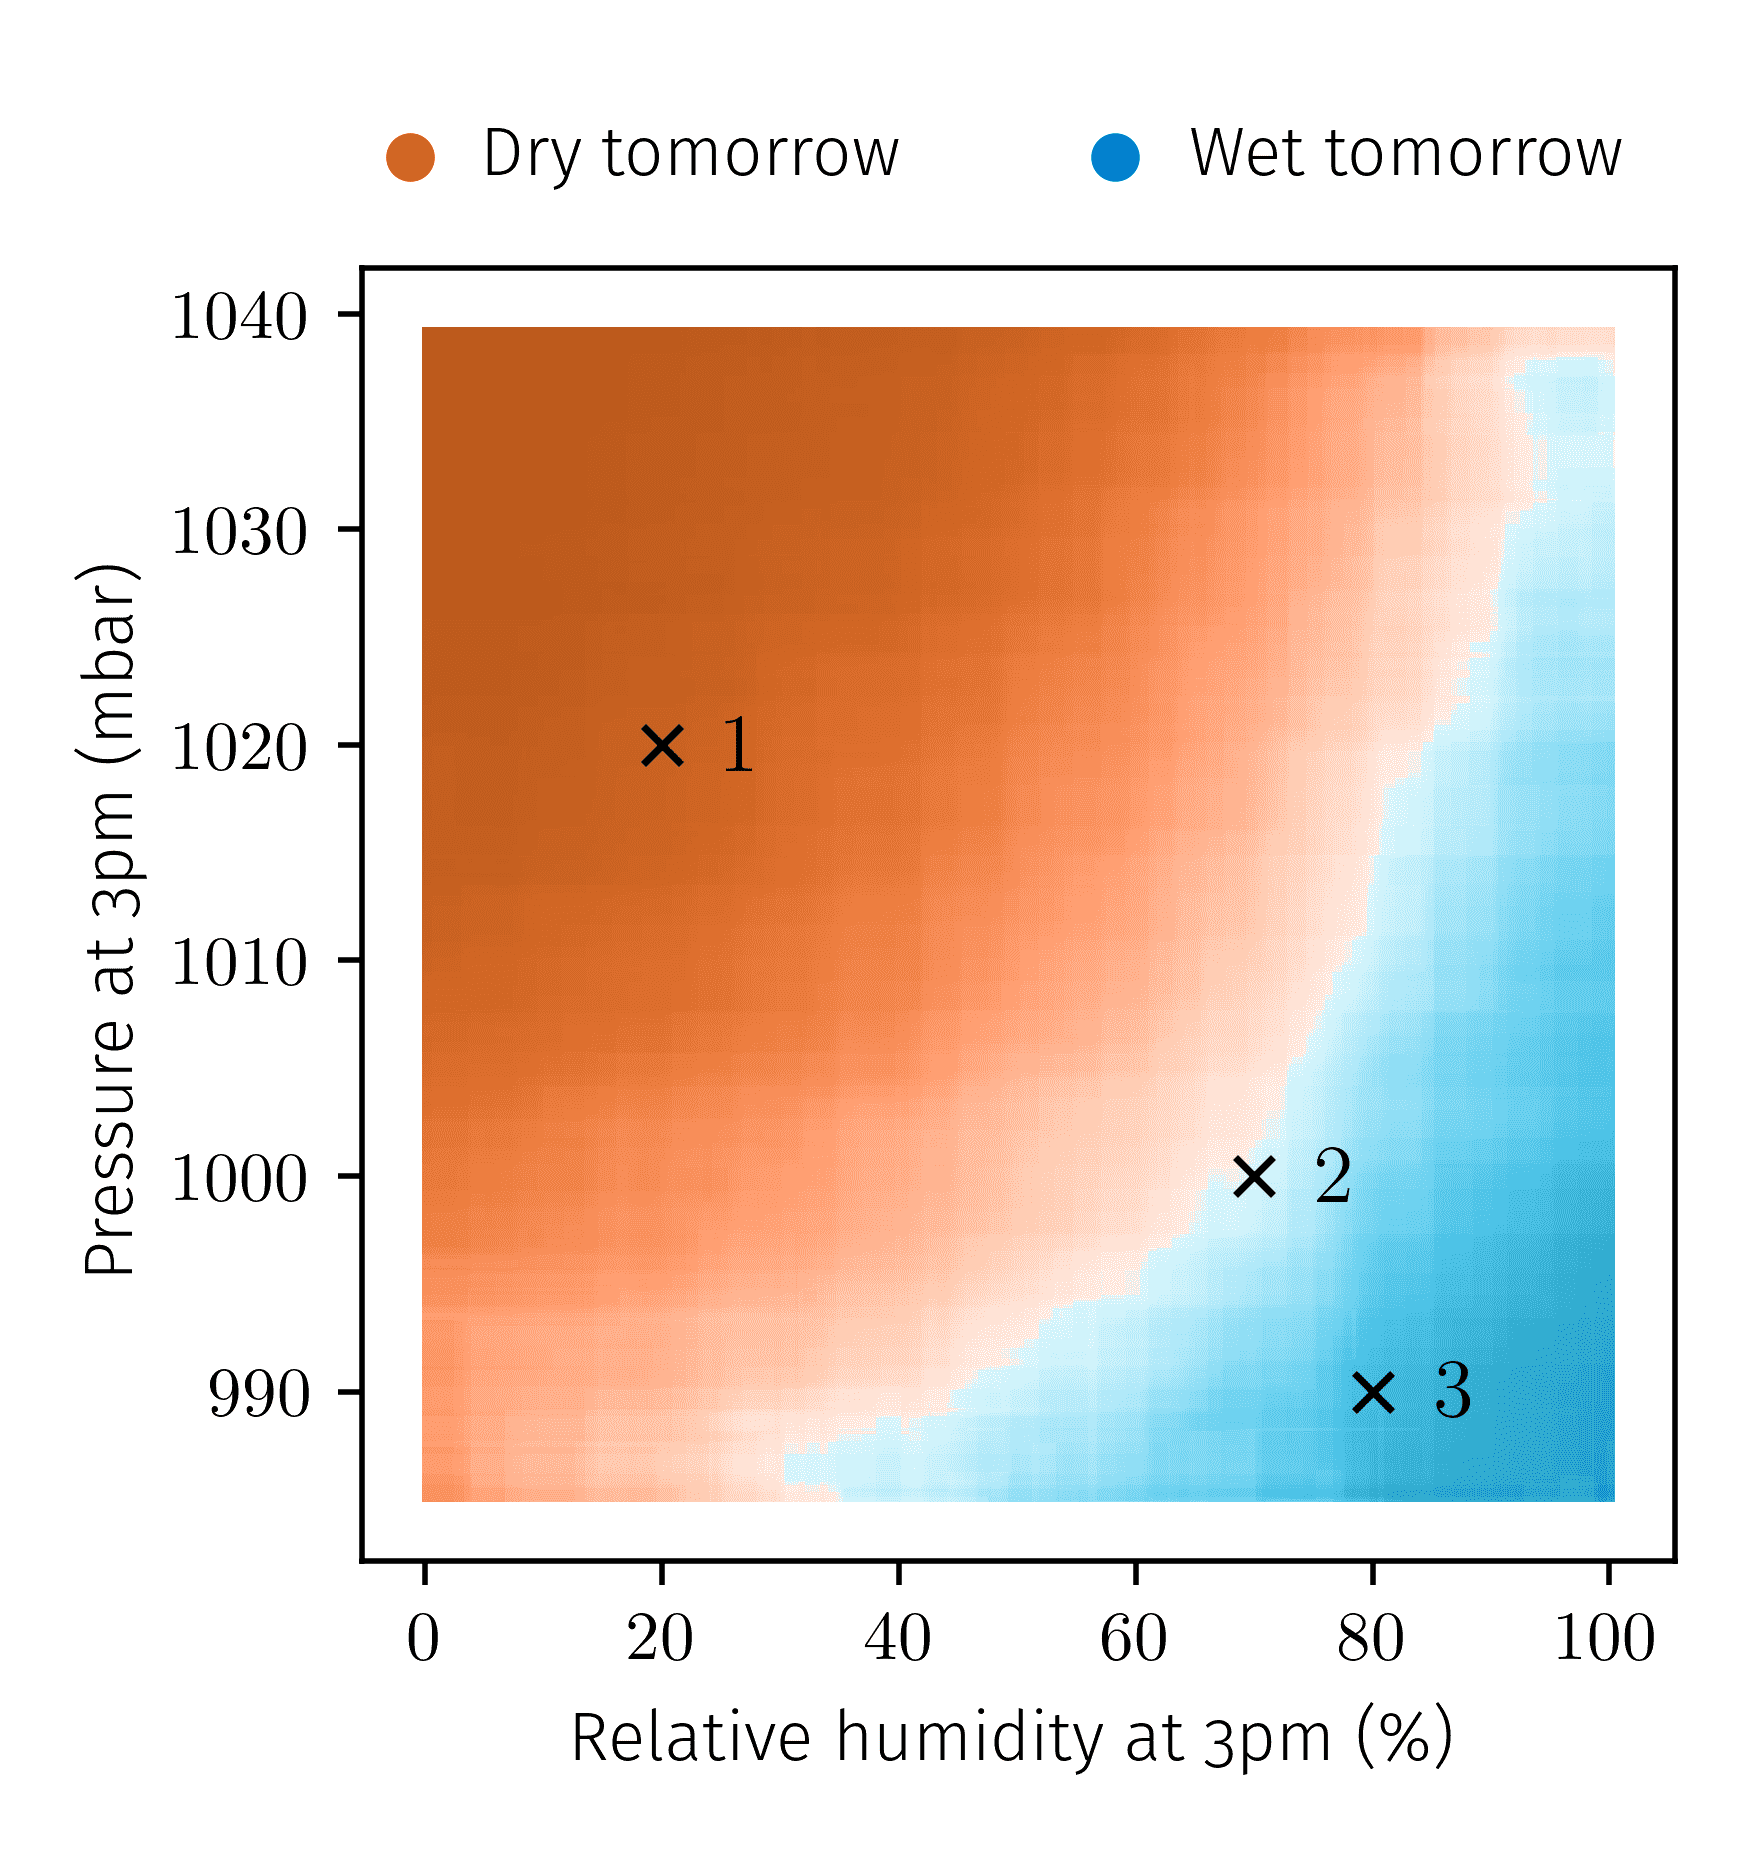
\includegraphics[scale=0.6]{
      graphics/weather_forest_design.png}%
    \end{subfigure}
  \end{figure}

  \vspace*{-8mm}
  \footnotesize{
    \begin{table}
      \begin{center}
        \begin{tabular}{|c|c|r|c|c|}
          \hline
          \textbf{Point} & \textbf{Humidity} & \textbf{Pressure} &
          \textbf{Chance of rain} & \textbf{95\% confidence interval} \\
          \hline
          $1$ & $20\%$ & $1020\,\textrm{mbar}$ &
          \cellcolor{drycolor!40!white} $\phantom{0}4.3\%$ &
          \cellcolor{drycolor!40!white} \hspace*{-0mm}$4.1\%$ -- $4.6\%$ \\
          $2$ & $70\%$ & $1000\,\textrm{mbar}$ &
          \cellcolor{wetcolor!5!white} $53.0\%$ &
          \cellcolor{wetcolor!5!white} $52.0\%$ -- $54.0\%$ \\
          $3$ & $80\%$ & $990\,\textrm{mbar}$ &
          \cellcolor{wetcolor!30!white} $77.5\%$ &
          \cellcolor{wetcolor!30!white} $74.4\%$ -- $80.6\%$ \\
          \hline
        \end{tabular}
      \end{center}
    \end{table}
  }

\end{frame}

\begin{frame}{Conclusion and ongoing work}

  \vspace*{3mm}
  Contributions to studying the Mondrian random forest estimator

  \begin{itemize}
    \item Provided a novel \alert{central limit theorem} allowing
      fully feasible \alert{statistical inference}
      via variance estimation
    \item Presented a new \alert{debiasing procedure} allowing
      for inference under milder conditions
    \item Demonstrated \alert{minimax optimality}
      for arbitrary dimension and smoothness,
      the first result for any forest estimator
  \end{itemize}

  Ongoing and future work

  \begin{itemize}
    \item Heterogeneous and data-dependent lifetimes
      $\hat \lambda_j$ or $\hat \lambda(x)$
    \item Improved estimation with additive models or local regression
    \item Uniform inference via strong approximation
  \end{itemize}

\end{frame}

\begin{frame}[noframenumbering,plain]
  \sectionpage
  \begin{center}
    \vspace*{8mm}
    \Large{\textbf{Uniform Inference for Kernel Density Estimators
    with Dyadic Data}} \\
    \vspace*{15mm}
    \normalsize{With Matias D.\ Cattaneo and Yingjie Feng}
  \end{center}
\end{frame}

\begin{frame}{Dyadic data}

  \begin{textblock*}{68mm}(60mm,20mm)
    \vspace*{1mm}
    Example of dyadic data
    \vspace*{-1mm}
    \begin{itemize}
      \item $A_i$ is GDP of country $i$
      \item $W_{i j}$ is value of trade $i \leftrightarrow j$
    \end{itemize}
  \end{textblock*}

  \begin{figure}
    \centering
    \hspace*{-60mm}
    \begin{subfigure}{0.54\textwidth}
      \centering
      \visible<1->{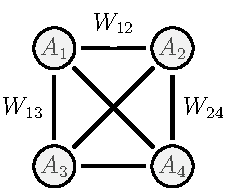
\includegraphics[scale=1.1]{graphics/network.pdf}}%
    \end{subfigure}
  \end{figure}

  \begin{itemize}

    \item
      $W_{i j}$ random variables associated with edges of a network

    \item Write $W_{i j} = W(A_i, A_j, V_{i j})$
      by Aldous--Hoover
      with $A_i$ latent node variables
      and $V_{i j}$ latent idiosyncratic shocks

    \item
      Unknown Lebesgue density $f(w)$ estimated by $\hat f(w)$
      on $\cW$

    \item
      We provide the \alert{minimax-optimal estimation} rate for $\hat f(w)$

    \item
      \alert{Uniform inference} on $f(w)$
      by strong approximation

  \end{itemize}

\end{frame}

\begin{frame}{Dyadic kernel density estimation}

  \vspace*{4mm}
  \begin{block}{Dyadic kernel density estimator}
    \vspace*{-4mm}
    %
    \begin{align*}
      \hat f(w)
      &= \frac{2}{n(n-1)}
      \sum_{i=1}^{n-1} \sum_{j=i+1}^{n}
      \frac{1}{h} K\left(\frac{W_{i j} - w}{h}\right)
    \end{align*}
    %
    \vspace*{-4mm}
  \end{block}

  \begin{itemize}
    \item
      Bandwidth $h$ controls bias--variance tradeoff
    \item
      Higher-order boundary kernels $K$
      improve bias properties
    \item We analyze the U-statistic Hoeffding-type decomposition

      \vspace*{-5mm}
      \begin{align*}
        \hat f(w) - f(w)
        &=
        \underbrace{B(w)}_{\substack{\text{smoothing}
        \\ \text{bias}}}
        + \underbrace{L(w)}_{\text{i.i.d.\ average}}
        + \underbrace{E(w)}_{\substack{\text{conditional}
        \\ \text{i.n.i.d.\ average}}}
        + \underbrace{Q(w)}_{\text{U-statistic}}
      \end{align*}

      \vspace*{-1mm}

    \item $L(w)$, $E(w)$ and $Q(w)$ are mean-zero and orthogonal

  \end{itemize}
\end{frame}

\begin{frame}{Minimax-optimal uniform dyadic estimation}

  \vspace*{2mm}
  \begin{itemize}
    \item Using an order $p$ boundary kernel,
      if $f$ is $\beta$-H{\"o}lder then

      \vspace*{-4mm}
      \begin{align*}
        \sup_{w \in \cW} \big| B(w) \big|
        &\lesssim h^{p\wedge\beta}
        &\E\left[ \sup_{w \in \cW} |L(w)| \right]
        &\lesssim
        \frac{D}{\sqrt n} \\
        \E\left[ \sup_{w \in \cW} |E(w)| \right]
        &\lesssim \sqrt{\frac{\log n}{n^2h}}
        &\E\left[ \sup_{w \in \cW} |Q(w)| \right]
        &\lesssim \frac{1}{n}
      \end{align*}

    \item
      Optimize the bound with $p \geq \beta$ and
      $h \asymp \left( \frac{\log n}{n^2} \right)^{\frac{1}{2 \beta + 1}}$

    \item Then we attain the minimax dyadic estimation rate
  \end{itemize}

  \vspace*{3mm}

  \begin{theorem}[Minimax-optimal uniform dyadic estimation]
    %
    \vspace*{-3mm}
    \small{
      \begin{align*}
        \sup_{w \in \cW}
        \big|\hat f(w) - f(w)\big|
        &\lesssim_\P
        \underbrace{h^{p \wedge \beta}\vphantom{\frac{D}{\sqrt n}}
        }_{\textcolor{alertcolor}{B(w)}}
        + \underbrace{\frac{D}{\sqrt n}
        }_{\textcolor{alertcolor}{L(w)}}
        + \underbrace{\sqrt{\frac{\log n}{n^2h}}\vphantom{\frac{D}{\sqrt n}}
        }_{\textcolor{alertcolor}{E(w)}}
        \lesssim
        \frac{D}{\sqrt n}
        + \left( \frac{\log n}{n^2} \right)^{\frac{\beta}{2\beta + 1}}
      \end{align*}
    }
    \vspace*{-4mm}
    %
  \end{theorem}

\end{frame}

\begin{frame}{Dyadic strong approximation construction}

  \begin{itemize}
    \item Need distributional approximations for both $L(w)$ and $E(w)$
    \item No uniform central limit theorem as $E(w)$ is not tight
    \item For the i.i.d.\ sum $L(w)$, use KMT coupling
      \citep{komlos1975approximation}
      \begin{align*}
        \sup_{w \in \cW} \left|\sqrt n L(w) - Z_L(w)\right|
        &\lesssim_\P
        \frac{D \log n}{\sqrt n}
      \end{align*}
    \item $E(w)$ is a sum of $\binom{n}{2}$
      conditionally independent but not i.i.d.\ terms
      so use a version of Yurinskii's coupling
      \citep{yurinskii1978error}
      \begin{align*}
        \sup_{w \in \cW} \left|\sqrt{n^2 h} E(w) - Z_E(w)\right|
        &\lesssim_\P
        \frac{(\log n)^{3/8}}{n^{1/4} h^{3/8}}
      \end{align*}
      %
    \item Combine these with the uniform bounds on $B(w)$ and $Q(w)$
  \end{itemize}

\end{frame}

\begin{frame}{Dyadic uniform inference via strong approximation}

  \vspace*{2mm}
  \begin{theorem}[Strong approximation and uniform confidence bands]
    %
    \vspace*{-3mm}
    \small{
      \begin{align*}
        \sup_{w \in \cW}
        \left|
        \frac{\hat f(w) - f(w)}{\sqrt{\Var\big[\hat f(w)\big]}}
        - Z(w)
        \right|
        &\to_\P 0,
        &&Z(w) \text{ Gaussian process}
      \end{align*}
    }
    \vspace*{-4mm}
    %
    \small{
      \begin{align*}
        \P\left(
          f(w)
          \in
          \left[
            \hat f(w)
            \pm
            \hat q_{1-\alpha}
            \sqrt{\widehat\Var\big[\hat f(w)\big]}
          \,\right] \
          \forall w \in \cW
        \right)
        \to
        1 - \alpha
      \end{align*}
    }
    \vspace*{-5mm}
    %
  \end{theorem}

  \vspace*{-2mm}
  \begin{figure}[H]
    \centering
    \begin{subfigure}{0.49\textwidth}
      \centering
      \visible{
        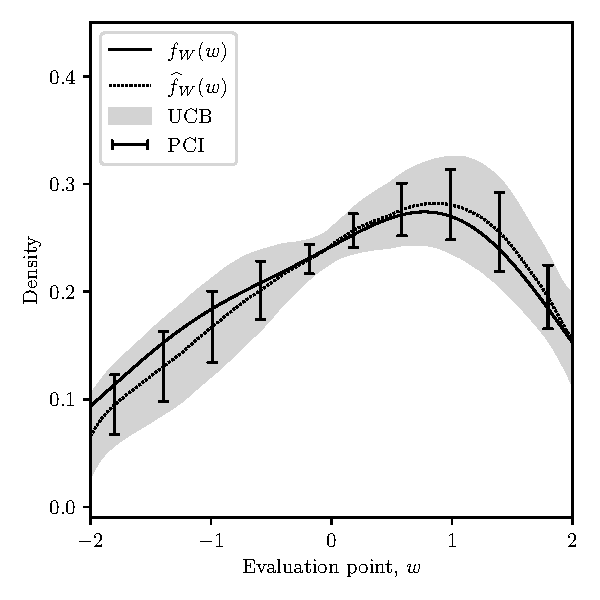
\includegraphics[scale=0.35]{graphics/result_partial.pdf}
        \vspace*{-3mm}
        \caption{
          Synthetic data with degeneracy
      }}
    \end{subfigure}
    %
    \begin{subfigure}{0.49\textwidth}
      \centering
      \visible{
        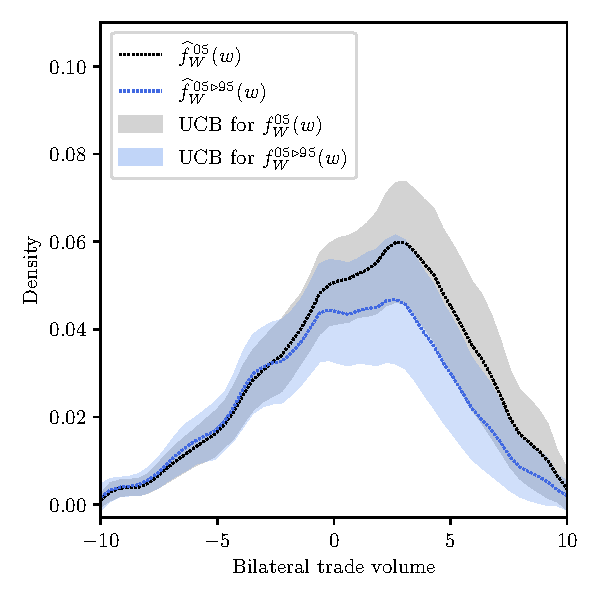
\includegraphics[scale=0.35]{graphics/trade_plot_1995_2005.pdf}
        \vspace*{-3mm}
        \caption{
        Counterfactual trade analysis}
      }
    \end{subfigure}
  \end{figure}

\end{frame}

\begin{frame}{Questions}

  \begin{minipage}{0.20\textwidth}
    \begin{figure}[ht]
      \centering
      \hspace*{-3mm}%
      
\includegraphics[width=0.99\textwidth]{graphics/logo_mondrian.png}%
      \hspace*{0mm}%
    \end{figure}
  \end{minipage}
  \begin{minipage}{0.79\textwidth}
    \footnotesize{
      Cattaneo, M.\ D.,
      Klusowski, J.\ M.,
      and Underwood, W.\ G.\ (2023) \\
      Inference with Mondrian random forests \\
      \href{https://arxiv.org/abs/2310.09702}%
      {\texttt{arXiv:2310.09702}} \\
      \href{https://github.com/WGUNDERWOOD/MondrianForests.jl}%
      {\texttt{github.com/wgunderwood/MondrianForests.jl}}
    }
  \end{minipage}

  \vspace{2mm}

  \begin{minipage}{0.20\textwidth}
    \begin{figure}[ht]
      \centering
      \hspace*{-3mm}%
      
\includegraphics[width=0.99\textwidth]{graphics/logo_dyadic.png}%
      \hspace*{0mm}%
    \end{figure}
  \end{minipage}
  \begin{minipage}{0.79\textwidth}
    \footnotesize{
      Cattaneo, M.\ D.,
      Feng, Y.,
      and Underwood, W.\ G.\ (2024). \\
      Uniform inference for kernel density estimators with dyadic data \\
      \href{https://arxiv.org/abs/2201.05967}%
      {\texttt{arXiv:2201.05967}} \\
      \href{https://github.com/WGUNDERWOOD/DyadicKDE.jl}%
      {\texttt{github.com/wgunderwood/DyadicKDE.jl}}
    }%
  \end{minipage}

\end{frame}

\appendix

\begin{frame}[allowframebreaks,noframenumbering]{References}
  \bibliographystyle{apalike}
  \renewcommand{\bibsection}{}
  \footnotesize{\bibliography{refs}}
\end{frame}

\endNoHyper
\end{document}

